\chapter{Reprezentacja i klasyfikacja utworu muzycznego}

Na rysunku 18 została przedstawiona gama chromatyczna rozpoczynająca się od dźwięku C:
\begin{figure}[H]
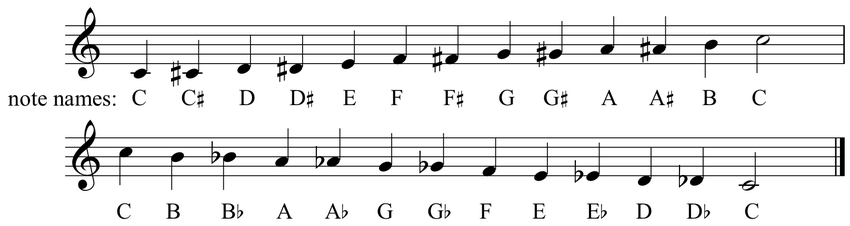
\includegraphics[scale = 0.4]{chromatyczna.png}
\centering
\caption{Skala dwunastodźwiękowa zwana także  \textit{chromatyczną}. Skala chromatyczna to skala, w której poszczególne stopnie oddalone są od siebie o pół tonu. Zawiera wszystkie dźwięki w obrębie danej oktawy, czyli łącznie 12 dźwięków. Krzyżyki oznaczają ruch w górę, bemole ruch w dół. Źródło: \url{https://www.researchgate.net/figure/Chromatic-scale-starting-with-C-22_fig1_334131988}}
\centering
\end{figure}
Skali chromatycznej odpowiada dowolny dwunastowymiarowy wektor wartości formatu \textit{MIDI}. Dla przykładu skala chromatyczna rozpoczynająca się od dźwięku (C, 4), a kończąca się na dźwięku (C, 5), to wektor:
\begin{equation*}
v =
\begin{bmatrix}
60,61,62,63,64,65,66,67,68,69,70,71
\end{bmatrix}
\text{gdzie} \quad v \in \mathbb{R}^{12}.
\end{equation*}

W analogiczny sposób można rozpisać dowolną gamę jako wektor wartości z których każda należy do przestrzeni liczb rzeczywistych. Należy jedynie pamiętać o tym, że wartości liczbowe poszczególnych dźwięków w formacie MIDI różnią się  w zależności of wybranej oktawy i należy je rozpisać zgodnie z powyższą klawiaturą MIDI.



\section{Implementacja zadania klasyfikacji dźwięków}

Stworzona w języku \textit{Haskell} biblioteka \textit{Euterpea}\footnote{https://www.euterpea.com/} pozwala w prosty sposób generować utwory muzyczne. Wykorzystuję się ją szeroko w muzyce algorytmicznej, analizie muzyki i syntezie dźwięku.

\textit{Euterpea} tworzy dźwięki przesyłając komunikaty MIDI do urządzenia, który jest w stanie je odczytać. W najprostszym przypadku takim urządzeniem może być programowy syntezator dźwięku \citep{Obrebski2020}

Prezentowany przeze mnie prosty program w języku Haskell dokonuje klasyfikacji dźwięków, wykorzystując przy tym fragmenty dwóch gotowych utworów muzycznych: 

\begin{enumerate}
    \item Pierwszy utwór \textit{Od Pilicy i Wolbroma} jest przedstawicielem muzyki ludowej i został udostępiony przez Instytut im. Oskara Kolberga (zob. Rysunek 18),
    \item Utwór \textit{Simple Jazz} pobrany z serwisu MuseScore (zob. Rysunek 19).
\end{enumerate}


\begin{figure}[H]
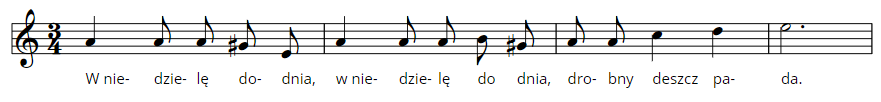
\includegraphics[scale = 0.8]{ludowa.png}
\centering
\caption{Utwór "Od Pilicy i Wolbroma", Źródło: \href{http://oskarkolberg.pl/pl-PL/MusicDb/Details/cafbb535-ed69-4b99-9002-f65fe40ed8fe}{Instytut im. Oskara Kolberga}}
\centering
\end{figure}

Pierwszemu utworowi odpowiada wektor:
\begin{equation*}
    v =
    \begin{bmatrix}
    69,69,69,68,64,69,69,69,71,68,69,69
    \end{bmatrix}
\end{equation*}

\begin{figure}[H]
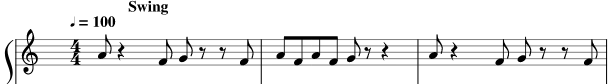
\includegraphics[scale = 0.8]{jazz.png}
\centering
\caption{Fragment utworu "Simple Jazz", Źródło: \href{https://musescore.com/user/27009977/scores/5429135}{Musescore.com}}
\centering
\end{figure}
Drugiemu utworowi odpowiada wektor $u$:
\begin{equation*}
u =
    \begin{bmatrix}
    69,65,67,65,69,65,69,65,67,71,65,67
    \end{bmatrix}
\end{equation*}

Funkcje dokonujące obliczeń zostały zadeklarowane w następujący sposób:
\begin{lstlisting}[language = Haskell]
-- odejmowanie dwoch wektorow
odejmij :: [Float] -> [Float] -> [Float]
odejmij [] _ = []
odejmij _ [] = []
odejmij (x:xs) (y:ys) = x - y : (odejmij xs ys)


-- Iloczyn skalarny
dot :: [Float] -> [Float] -> Float
dot x y = sum $ zipWith (*) x y

klasyfikacja:: Float -> Int
klasyfikacja y_x
    | y_x > w_0 = 1 -- klasa C1
    | y_x < w_0 = -1 --klasa C2

toAbsPitches :: [Pitch] -> [AbsPitch]
toAbsPitches ps = map absPitch ps


toPitches :: [AbsPitch] -> [Pitch]
toPitches as = map pitch as
\end{lstlisting}

Pomocnicze funkcje \textit{ToPitches} i \textit{toAbsPitches} umożliwiają konwersje z  zapisu nutowego do liczb całkowitych i odwrotnie \citep[s. 60]{HSOM_2018}.

Klasyfikacje możemy przeprowadzić na dwa sposoby:
\begin{itemize}
    \item Na podstawie podobieństwa poszczególnych dźwięków do siebie,
    \item Na podstawie mierzalnych cech, które opisują utwór muzyczny. W tym wypadku skupimy się na \textit{rytmie}.
\end{itemize}

\subsection{4.2 Klasyfikacja na podstawie podobieństwa dźwięków}
Mając dane dwa wektory $v$ i $u$, sprawdźmy, czy wektor $x$ jest bardziej podobny do muzyki ludowej ($C_{1}$), reprezentowanej przez wektor $v$, czy do muzyki jazzowej ($C_{2}$), reprezentowanej przez $u$. 

\begin{equation*}
v =
\begin{bmatrix}
69,69,69,68,64,69,69,69,71,68,69,69
\end{bmatrix}
\end{equation*}

\begin{equation*}
    u =
    \begin{bmatrix}
    69,65,67,65,69,65,69,65,67,71,65,67
    \end{bmatrix}
\end{equation*}

Jako pierwszy przykład testowy wykorzystamy fragment utworu \textit{The Entertainer} (zob.rys. 21) który zakodowaliśmy jako wektor $x$:
\begin{equation*}
x =
    \begin{bmatrix}
   60,60,60,60,60,60,62,63,60,62,64,64
    \end{bmatrix}
\end{equation*}

\begin{figure}[H]
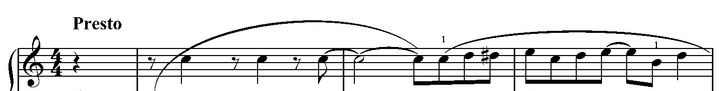
\includegraphics[scale = 0.7]{entertainer.png}
\centering
\caption{Fragment utworu "The Entertainer". Źródło: \url{https://www.8notes.com/scores/13178.asp}}
\centering
\end{figure}

Przebieg klasyfikacji przebiega następująco. Najpierw obliczamy $y$:
\begin{align*}
y = [(69 - 69), (69 - 65), (69 - 67), (68 - 65), \\ (64 - 69), 
(69 - 65), (69 - 69), (69 - 65),\\ (71 - 67), (68 - 71), (69 - 65), (69 - 67)].
\end{align*}

Zatem:
\begin{equation*}
y =  [0, 4, 2, 3, -5, 4, 0, 4, 4, -3, 4, 2].
\end{equation*}

Następnie obliczamy $w_{0}$:
\begin{align*}
w_{0} = &  \frac{1}{2} \big(\|v\|^{2} - \|u\|^{2}\big)  \\
= & \frac{1}{2}[(69 \cdot 69) + (69 \cdot 69) + (69 \cdot 69) + (68 \cdot 68) \\
 & + (64 \cdot 64) + (69 \cdot 69) + (69 \cdot 69) + (69 \cdot 69) \\
 & + (71 \cdot 71) + (68 \cdot 68)  + (69 \cdot 69) + (69 \cdot 69) \\
 - & (69 \cdot 69) + (65 \cdot 65) + (67 \cdot 67) + (65 \cdot 65) \\
 & + (69 \cdot 69) + (65 \cdot 65) + (69 \cdot 69) + (65 \cdot 65) \\
 & + (67 \cdot 67) + (71 \cdot 71) + (65 \cdot 65) + (67 \cdot 67)] \\
 = & \frac{1}{2}(56473 - 53916) \\
 = & \frac{1}{2}(2557) = 1278,5.
\end{align*}
Wtedy:
\begin{align*}
\big \langle y|x  \big \rangle  = \quad 
& [0, 4, 2, 3, -5, 4, 0, 4, 4, -3, 4, 2] \\ 
&\cdot
[60,60,60,60,60,60,62,63,60,62,64,64] 
= 1170.
\end{align*}
Jeśli, $\big \langle y|x \big \rangle < w_{0}$, to $f(x) = -1$, a to oznacza przydział do klasy $C_{2}$.

Klasyfikator uznał zatem, że dźwięki w wektorze $x$ są bardziej podobne do tych w wektorze $u$. Bluesowy utwór \textit{The Entertainer} został uznany za bardziej podobny do jazzu niż do muzyki ludowej, co raczej zgadza się z powszechną intuicją Ten sposób klasyfikacji nie jest optymalny, ponieważ pomija wszystkie inne cechy utworu, takie jak \textit{rytm}. W kolejnym podrozdziale pokażemy jak można rozwiązać ten problem i zamodelujemy klasyfikacje na podstawie rytmu.

\section{Modelowanie binarne typu cisza - dźwięk}

Sposobem na klasyfikacje utworów względem ich rytmu jest takie zamodelowanie wektora wejściowego nut, gdzie do każdej wartości dźwiękowej, (nie będącej pauzą), przyporządkowujemy wartość 1, a każdej wartości będącej pauzą przyporządkowujemy wartość 0. Przyporządkowanie to zawsze działa w taki sam sposób, niezależnie od tego jakiej długości jest dana nuta, czy pauza. Prosty przykład jak miałoby to wyglądać został przedstawiony na rys. 20.

\begin{figure}[H]
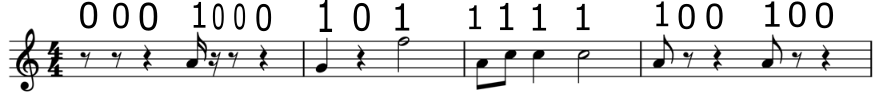
\includegraphics[scale = 0.5]{test.png}
\centering
\caption{Przykład binarnego modelowania na pięciolinii. Wartość "1" przyporządkowujemy jedynie dźwiękom, niezależnie od długości i trwania, a wartość "0" zostawiamy dla pauz. Źródło: Opracowanie własne w programie \textit{MuseScore} i \textit{Inkscape}.}
\centering
\end{figure}

Powiedzieliśmy sobie wcześniej, że rytm jest zmienną odpowiedzialną za czasową organizacje przebiegu utworu. Zbudowanie wektora nut w taki sposób da nam możliwość śledzenia ile występuje pauz i dźwięków i w jakiej one są kolejności, a dzięki temu będziemy mieli możliwość porównywania utworów pod względem ich struktury. Takie rozwiązanie sprawia, że uzyskujemy więcej informacji o melodii, niż miało to miejsce w przypadku porównywania samych dźwięków, bez uwzględniania ich kolejności.
Wykorzystamy tym razem próbkę złożoną z 21 wartości dźwięków i pauz, żeby badane wektory $v$, $u$ oraz $x$ zgadzały się ze sobą pod względem wymiarów.

Na początku ustalmy wektory $v$, $u$ oraz $x$
\begin{equation*}
    v = 
    \begin{bmatrix}
    1,0,1,1,1,1,1,0,1,1,1,1,1,1,1,1,1,0,1,1,1
    \end{bmatrix}
\end{equation*}

\begin{equation*}
    u =
    \begin{bmatrix}
    1,0,1,1,0,0,1,1,1,1,1,1,0,0,1,0,1,1,0,0,1
    \end{bmatrix}
\end{equation*}

\begin{equation*}
    x =
    \begin{bmatrix}
    0,1,0,1,0,1,1,1,1,1,1,1,1,1,1,1,1,1,1,1,1
    \end{bmatrix}
\end{equation*}

Na tej podstawie dokonujemy klasyfikacji.
Zatem:
\begin{equation*}
    y = v - u =
    \begin{bmatrix}
    0,0,0,0,1,1,0,-1,0,0,0,0,1,1,0,1,0,-1,1,1,0
    \end{bmatrix}
\end{equation*}
Następnie:

\begin{equation*}
w_{0} =\frac{1}{2} \big(\|v\|^{2} - \|u\|^{2}\big) = 2.5.
\end{equation*}
Wtedy:
\begin{equation*}
\big \langle y|x  \big \rangle = 2.0.
\end{equation*}
Stąd:
\begin{equation*}
    \big \langle y|x \big \rangle < w_{0}, \quad \text{wtedy} \quad f(x) = -1
\end{equation*}
A to również oznacza przydział do klasy $C_{2}$.
Zatem klasyfikując na podstawie rytmu program ponownie uznał, że bluesowy utwór \textit{The Entertainer} brzmi bardziej jazzowo niż ludowo.

\subsection{4.4 Procedura testowa}
Na podstawie powyżej opisanych dwóch metod przeprowadzono testy dla większej ilości utworów. Przebieg procedury testowania był następujący:
\begin{enumerate}
    \item Wygenerowanie losowego wektora $x$,
    \item Obliczenie $y = v - u$,
    \item Obliczenie wartości $w_{0} =\frac{1}{2} \big(\|v\|^{2} - \|u\|^{2}\big)$,
    \item Obliczenie $\big \langle y|x \big \rangle$,
    \item Przydział wektora $x$ do klasy $C_{1}$ lub $C_{2}$.
\end{enumerate}

Jako, że wzorcowe wektory $v$ i $u$ zostały wprowadzone jako wartości całkowite, a do obliczenia iloczynu skalarnego potrzebujemy listy wartości zmiennoprzecinkowych, to ich konwersja na typ \textit{Float} została przeprowadzona przy pomocy funkcji \textit{floatList} zaimplementowanej następująco

\begin{lstlisting}[language = Haskell]

-- Konwersja listy int na float
floatList :: [AbsPitch] -> [Float]
floatList [] = []
floatList (n:ns)  = (x) : floatList(ns)
    where x = fromIntegral n :: Float 
\end{lstlisting}

Testy przeprowadzono w dwóch wariantach. W wariancie pierwszym (A) porównywano wektor wzorcowy danego typu muzyki (ludowej bądź jazzowej), z innym utworem z tego samego gatunku muzyki. Przykłady zostały pobrane z seriwsu \textit{MuseScore} lub z \textit{Instytutu im. Oskara Kolberga}, odpowiednio 5 utworów muzyki ludowej lub jazzowej. W wariancie (B) wektory wzorcowe były porównywane z losowo wygenerowanym innym wektorem, żeby sprawdzić jakie decyzje podejmuje algorytm dla losowo wygenerowanych sekwencji dźwięków. 

\subsection{(A) Porównywanie utworu wzorcowego z innym utworem}
\FloatBarrier
\begin{table}[h]
\centering
\begin{tabular}{|c|c|c|}
\hline
Lp. & $X_{input}$ & $X_{output}$ \\ \hline
1.   & $C_{1}$      & $C_{2}$      \\ \hline
2.   & $C_{1}$      & $C_{1}$     \\ \hline
3.   & $C_{1}$      & $C_{2}$      \\ \hline
4.   & $C_{1}$      & $C_{1}$     \\ \hline
5.   & $C_{1}$      & $C_{1}$      \\ \hline
6.   & $C_{2}$      & $C_{2}$    \\ \hline
7.   & $C_{2}$      & $C_{2}$     \\ \hline
8.   & $C_{2}$      & $C_{2}$     \\ \hline
9.   & $C_{2}$      & $C_{1}$     \\ \hline
10.  & $C_{2}$      & $C_{2}$      \\ \hline
\end{tabular}
\caption{Wyniki klasyfikacji na podstawie podobieństwa dźwięków. Źródło: Opracowanie własne.}
\end{table}
\FloatBarrier

\textbf{Podsumowanie:}
Wyniki klasyfikacji na podstawie podobieństwa dźwięków kształtują się następująco:

\begin{enumerate}
    \item Dla muzyki ludowej klasyfikator osiągnął 60\% dokładności (2 z 5 utworów zaklasyfikowano źle)
    \item Dla muzyki jazzowej klasyfikator osiągnął 80\% dokładności (1 z 5 utworów zaklasyfikowano źle)
\end{enumerate}

\textbf{Łącznie dla 10 przypadków, 7 razy dokonano poprawnej klasyfikacji (70\% dokładności)}.
\FloatBarrier
\begin{table}[h]
\begin{tabular}{|c|c|c|}
\hline
Lp. & $X_{input}$ & $X_{output}$ \\ \hline
1.   & $C_{1}$      & $C_{1}$      \\ \hline
2.   & $C_{1}$      & $C_{1}$     \\ \hline
3.   & $C_{1}$      & $C_{1}$      \\ \hline
4.   & $C_{1}$      & $C_{1}$     \\ \hline
5.   & $C_{1}$      & $C_{1}$      \\ \hline
6.   & $C_{2}$      & $C_{2}$    \\ \hline
7.   & $C_{2}$      & $C_{2}$     \\ \hline
8.   & $C_{2}$      & $C_{1}$     \\ \hline
9.   & $C_{2}$      & $C_{2}$     \\ \hline
10.  & $C_{2}$      & $C_{2}$      \\ \hline
\end{tabular}
\centering
\caption{Wyniki klasyfikacji na podstawie podobieństwa rytmu. Źródło: Opracowanie własne.}
\end{table}
\FloatBarrier

\textbf{Podsumowanie:}
Wyniki klasyfikacji na podstawie podobieństwa rytmu kształtują się następująco:

\begin{enumerate}
    \item Dla muzyki ludowej klasyfikator osiągnął 100\% dokładności (0 z 5 utworów zaklasyfikowano źle)
    \item Dla muzyki jazzowej klasyfikator osiągnął 90\% dokładności (1 z 5 utworów zaklasyfikowano źle)
\end{enumerate}

\textbf{Łącznie dla 10 przypadków, 9 razy dokonano poprawnej klasyfikacji (90\% dokładności)}.





\subsection{(B) Porównywanie utworu wzorcowego z utworem losowym}

Generowanie losowego wektora nut przeprowadzono za pomocą monady zaimplementowanej w następujący sposób:
\begin{lstlisting}[language = Haskell]

import System.Random (randomRIO) 
-- funkcje generujace listy 
randomFloat :: Float -> IO([Float])
randomFloat 0 = return []
randomFloat n = do
  r  <- randomRIO (20, 108) -- zakres
  rs <- randomFloat (n-1) -- generuje liste
  return (r:rs)
  
randomBin :: Int -> IO([Int])
randomBin 0 = return []
randomBin n = do
    r <- randomRIO (1,0) -- zakres
    rs <- randomBin (n-1)
    return (r:rs)
\end{lstlisting}

Funkcja \textit{randomFloat} generuje wektor wartości dźwiękowych o dowolnej długości, zakres losowania zmieniał się co iteracje i został ustalony na przedział 20 - 108, co odpowiada zakresowi wartości formatu \textit{MIDI}. Funkcja \textit{randomBin} generuje wektor złożony z zer i jedynek, również o dowolnej długości.
\FloatBarrier
\begin{table}[h]
\begin{tabular}{|c|c|c|}
\hline
Lp. & $X_{input}$ & $X_{output}$ \\ \hline
1.   & $C_{1}$      & $C_{1}$      \\ \hline
2.   & $C_{1}$      & $C_{2}$     \\ \hline
3.   & $C_{1}$      & $C_{1}$      \\ \hline
4.   & $C_{1}$      & $C_{1}$     \\ \hline
5.   & $C_{1}$      & $C_{1}$      \\ \hline
6.   & $C_{2}$      & $C_{1}$    \\ \hline
7.   & $C_{2}$      & $C_{2}$     \\ \hline
8.   & $C_{2}$      & $C_{2}$     \\ \hline
9.   & $C_{2}$      & $C_{2}$     \\ \hline
10.  & $C_{2}$      & $C_{1}$      \\ \hline
\end{tabular}
\centering
\caption{Wyniki klasyfikacji na podstawie podobieństwa dźwięków dla wektorów losowych. Źródło: Opracowanie własne.}
\end{table}
\FloatBarrier

\textbf{Podsumowanie:}
Wyniki klasyfikacji na podstawie podobieństwa rytmu kształtują się następująco:

\begin{enumerate}
    \item Dla muzyki ludowej klasyfikator osiągnął 80\% dokładności (1 z 5 utworów zaklasyfikowano źle)
    \item Dla muzyki jazzowej klasyfikator osiągnął 60\% dokładności (2 z 5 utworów zaklasyfikowano źle)
\end{enumerate}

\textbf{Łącznie dla 10 przypadków, 7 razy dokonano poprawnej klasyfikacji (70\% dokładności)}.
\FloatBarrier
\begin{table}[h]
\begin{tabular}{|c|c|c|}
\hline
Lp. & $X_{input}$ & $X_{output}$ \\ \hline
1.   & $C_{1}$      & $C_{1}$      \\ \hline
2.   & $C_{1}$      & $C_{2}$     \\ \hline
3.   & $C_{1}$      & $C_{2}$      \\ \hline
4.   & $C_{1}$      & $C_{2}$     \\ \hline
5.   & $C_{1}$      & $C_{2}$      \\ \hline
6.   & $C_{2}$      & $C_{2}$    \\ \hline
7.   & $C_{2}$      & $C_{2}$     \\ \hline
8.   & $C_{2}$      & $C_{1}$     \\ \hline
9.   & $C_{2}$      & $C_{1}$     \\ \hline
10.  & $C_{2}$      & $C_{2}$      \\ \hline
\end{tabular}
\centering
\caption{Wyniki klasyfikacji na podstawie podobieństwa rytmu dla wektorów losowych. Źródło: Opracowanie własne.}
\end{table}
\FloatBarrier

\textbf{Podsumowanie:}
Wyniki klasyfikacji na podstawie podobieństwa rytmu kształtują się następująco:

\begin{enumerate}
    \item Dla muzyki ludowej klasyfikator osiągnął 10\% dokładności (4 z 5 utworów zaklasyfikowano źle)
    \item Dla muzyki jazzowej klasyfikator osiągnął 40\% dokładności (3 z 5 utworów zaklasyfikowano źle)
\end{enumerate}

\textbf{Łącznie dla 10 przypadków, 3 razy dokonano poprawnej klasyfikacji (30\% dokładności)}.

\section{Wnioski}

Najlepsze wyniki klasyfikacji osiągnięto podczas testowania na utworach rzeczywistych. Algorytm osiągał porównywalnie gorsze wyniki w wariancie z utworami generowanymi losowo. Klasyfikacja na podstawie podobieństwa dźwięków osiągała gorsze wyniki niż klasyfikacja na podstawie rytmu dla utworów rzeczywistych, ale jej skuteczność znacznie się pogorszyła dla utworów generowanych losowo, co może oznaczać, że algorytm klasyfikacji faktycznie dobrze wykrywa rytm melodii. Głównym wnioskiem płynącym z badań jest teza, że klasyfikacja na podstawie rytmu jest dokładniejsza, ale żeby ją potwierdzić, bądź odrzucić należało by wykonać testy dla większej ilości przypadków testowych.
